\chapter{Implementation}
This chapter won't discuss, but report the actual building process for the 5S drifter and the final product 
up to a week before the final day of presentation. The Implementation step will be divided into hardware;
the protoboard construction and conection, and software; as how the planned algorith was coded.
\section{Hardware and Shell}

\subsection{Design alterations}

The waterfall modules states that, for better flow of work, it should'nt go back to previous steps 
and continue with minimal alterations. However, some alterations have to be made due to modules 
availability, since the planed modules where out of stock, and the team equipment was affected midway
the project. In order to deal with thease problems, modules were adapted (the modules shown in design 
chapter will cite the original module) as well to reduce the project scope even further to acomodate
the equipment available.  

\subsection{Voltage converter}

As the GNSS and LTE module differ in voltage from the uC, voltage alteration from the battery is needed.
As the module will work in two main voltages the GNSS module with 16V and the uC with 5V
, and there is no purpose tho isolate them, a Buck could be used to step down the 16V to 5V or a Bost to do 
it the other way around. As to minimize losses, the step down method was chosen using a LM2596 with 92\% 
efficiency.

\begin{figure}[H]
    \centering
    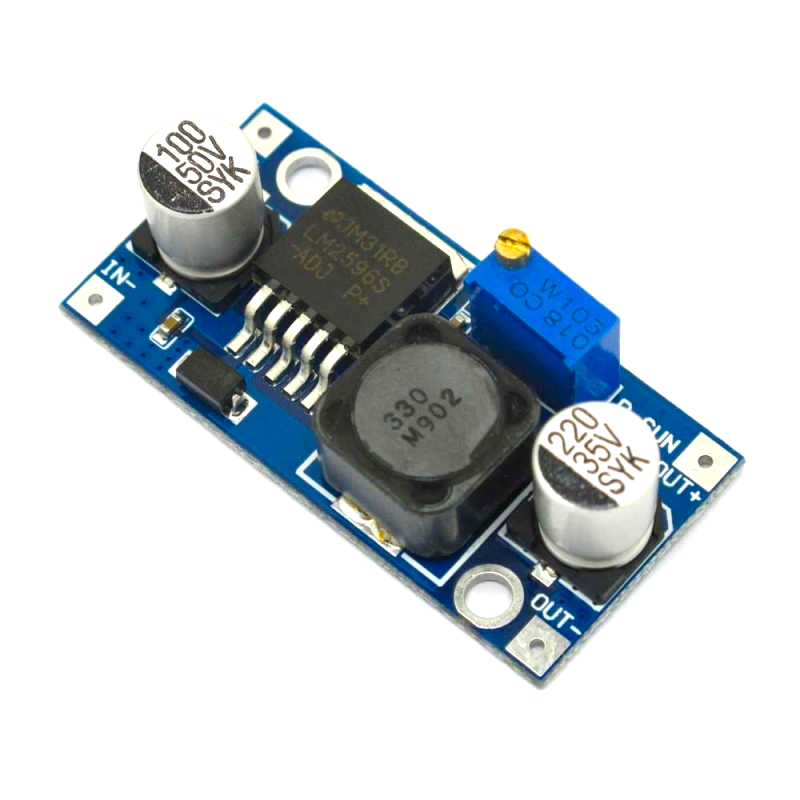
\includegraphics[width=0.3\textwidth]{images/chapter/implementation/step-sown.jpg}  % Adjust the width as necessary
    \caption{Step Down}
    \label{fig:Step Down}        
\end{figure}


\subsection{Final Shell Version}

The buoy was made on fusion360 and the model aproved by the laboratory personal. The project was done by the
design without any alterations, creating 4 final parts, 2 3D printed parts named as "Tip" holding the anthenna
in place and the temperature sensor under water, a 3D printed basket part holding the eletronics that will be
covered in plastic for waterproof the system, then at last, a non-printed buoy. 

The basket just takes in attention the space to hold the eletronics, then using the minimal distances it was
intersected at that hight and fixed there using nuts.
\begin{figure}[H]
    \centering
    
\includegraphics[width=1\textwidth]{images/chapter/implementation/Cesto.png}  % Adjust the width as necessary
    \caption{Shell Basket}
    \label{fig:Shell Basket}        
\end{figure}

The Tip will be printed twice, marking the pillas angle and fixed using zinc plated nut.
\begin{figure}[H]
    \centering
    
\includegraphics[width=1\textwidth]{images/chapter/implementation/ponta.png}  % Adjust the width as necessary
    \caption{Shell Tip}
    \label{fig:Shell Tip}        
\end{figure}

The models will be printed with 20\% infill to minimize weight and still have a good durability to inpact.
The boyant part is made from a specialized EPS available on laboratory used on the NEXTSEA and SONDA drifters.
The main pillars are made from zinc plated steel, as to resist the water oxidation.

\section{Software}
\subsection{Mobile Communication}
Along the Design step it was decided to use either Nb-Iot or LTE. Due to the low-power nature of Nb-Iot, 
it was primarily the main option. However, due to complications with the SIM provider, the protocol
switched to LTE as the SIMBASE SIM, available on lab, was compatible with the module. 

The SIMBASE offers a per day + per MB payiment subscription. Offering a plan for 0.01€ per day and 0.005€ per MB.
As previosly stated, the run time and amount of data generated is known. Sp the total cost fot he SIM, without the SIM itself
comes to;

\(Total = 0.01*4*30 + 0.005*3.4*1000 = 18.20\)

\subsection{AT commands}

AT commands (short for "Attention" commands) are a standardized set of instructions used to control modems
and communication modules such as GSM, LTE, and Wi-Fi. They are issued over a 
serial interface like UART (Universal Asynchronous Receiver/Transmitter) and typically start with the prefix
AT. The general structure includes different formats: AT alone to test communication, AT+COMMAND to execute
a command, AT+COMMAND? to read a parameter, AT+COMMAND=? to test availability, and AT+CO- 
-MMAND=value to set a parameter.

In order to further abstract the AT commands, as the list of commands needed is long, the folling wrapper is done.

\begin{lstlisting}[style=cStyle, caption={GNSS Power-On and Command Functions}]
    void at_power_on (char* received) //Abstracted function
    {
        gnss_sendCommand("AT+CGNSPWR=1\r\n", COMMAND_GENERAL_DELAY, received);
    //AT command with the right format, a delay and at 
    //last a pointer to a char array storing the result. 
    }
    
    void mobile_sendCommand(char * command, unsigned int timeout, char * received)
    {
        HAL_UART_Transmit_IT(MOBILE_COMMS_UART, command, strlen(command)); 
        //Transmits
        HAL_UART_Receive(MOBILE_COMMS_UART, received, 32, timeout); 
        //Reads the module
    }
    
    void gnss_sendCommand(char * command, unsigned int timeout, char * received)
    {
        HAL_UART_Transmit_IT(GNSS_UART, command, strlen(command)); 
        //Transmits
        HAL_UART_Receive(GNSS_UART, received, 32, timeout); 
        //Reads the module
    }
\end{lstlisting}
Communication over UART is done using ASCII text, with each AT command terminated by a 
carriage return (ASCII 0x0D), and often a line feed (ASCII 0x0A) depending on the module.

Timing is critical: commands should be sent with a small delay between them (typically 100–500 ms is safe), 
and you must wait for a response (like OK, ERROR, or data such as +CSQ: 15,0) before sending the next one. 
The baud rate (speed) of UART must match between your host and the module, commonly set to 9600 or 19200 bps. 
When using a microcontroller, the UART peripheral sends the commands as strings and waits for the module to 
reply.

Here are some of the AT commands that play critical role on the 5S Communication execution. Fisrt the commands
related to the GNSS communication, then the commands that control the LTE communication.

\begin{table}[h!]
    \centering
    \small
    \begin{tabular}{l|l}
        \textbf{AT Command} & \textbf{Function and Return Explanation} \\
        \hline
        \arrayrulecolor[gray]{0.85}
        \texttt{AT} & Basic command to check communication.\\ 
        & Returns \texttt{OK} if the module is responsive. \\
        \hline
        \texttt{AT+CGNSPWR?} & Queries GNSS power status.\\ 
        & Returns \texttt{+CGNSPWR: 0} (OFF) or \texttt{+CGNSPWR: 1} (ON). \\
        \hline
        \texttt{AT+CGNSPWR=1} & Turns ON the GNSS power. \\ 
        & Returns \texttt{OK} if successful. \\
        \hline
        \texttt{AT+CGNSINF} & Provides GNSS fix information.\\ 
        & Requires GNSS to be powered on. Return values like time, coordinates, speed, etc. \\
        \arrayrulecolor{black}
    \end{tabular}
    \caption{GNSS-Related AT Commands}
\end{table}

Further information on the +CGNSINF command, as it returns more options of information.

\begin{table}[h!]
    \centering
    \small
    \begin{tabular}{l|l}
        \textbf{Field} & \textbf{Parameter Description} \\
        \hline
        \arrayrulecolor[gray]{0.85}
        Run Status & Indicates if GNSS is powered: 0 = off, 1 = on \\
        \hline
        Fix Status & Fix validity: 0 = no fix, 1 = valid fix \\
        \hline
        UTC & Coordinated Universal Time in format YYYYMMDDHHMMSS.SSS \\
        \hline
        Latitude & Latitude in decimal degrees (North/South) \\
        \hline
        Longitude & Longitude in decimal degrees (East/West) \\
        \hline
        Altitude & Altitude in meters above sea level \\
        \hline
        Speed & Speed over ground in km/h \\
        \hline
        Course & Course over ground in degrees (0–360°) \\
        \hline
        Fix Mode & Positioning mode: 1 = Autonomous, 2 = DGPS, 3 = RTK \\
        \hline
        Reserved1 & Reserved (usually 0) \\
        \hline
        HDOP & Horizontal Dilution of Precision \\
        \hline
        PDOP & Position Dilution of Precision \\
        \hline
        VDOP & Vertical Dilution of Precision \\
        \hline
        Reserved2 & Reserved (usually 0) \\
        \hline
        Satellites in View & Number of satellites in view \\
        \hline
        GNSS Satellites Used & Number of satellites used for fix \\
        \hline
        GLONASS Satellites Used & Number of GLONASS satellites used \\
        \hline
        Reserved3 & Reserved (usually 0) \\
        \hline
        C/N0 max & Maximum carrier-to-noise ratio (dB-Hz) \\
        \hline
        HPA & Horizontal position accuracy estimate in meters \\
        \arrayrulecolor{black}
        \end{tabular}
    \caption{Detailed Breakdown of \texttt{+CGNSINF} Response Fields}
\end{table}
Once with the GNSS information, now the data has to be sent via LTE and received by the database 

The database communication won't be covered here, however, in order to prove the concept, a URL from the 
nextsea project is used. There are two links, one of them leads to a data.txt inside the nextsea server, 
the other writes on the data.txt. In order to prove the concept the prototype sends a formatted JSON file by the
second link, and it is visualized inside the data.txt. The JSON has the following components, following the 
package structure already established.
\\
\begin{lstlisting}[language=json]
    {
        "package_number": %d,
        "utl_time": %s,
        "power_level": %d,
        "temperature": [%f, %f, %f...],
        "imu": [%f, %f, %f...],
        "gnss": 
          [0, 0, 0]
        "errors": 0
      }
\end{lstlisting}

\begin{table}[H]
    \centering
    \small
    \begin{tabular}{l|l}
        \textbf{AT Command} & \textbf{Function and Return Explanation} \\
        \hline
        \arrayrulecolor[gray]{0.85}
        \texttt{AT+CPIN?} & Checks SIM card status. \\ 
        & Returns \texttt{+CPIN: READY} if SIM is present and unlocked. \\
        \hline
        \texttt{AT+CNMP=38} & Sets the network mode to LTE only. \texttt{38} = LTE. \\ 
        & Returns \texttt{OK}. \\
        \hline
        \texttt{AT+CMNB=3} & Configures LTE category to CAT-M1 only. \\ 
        & Returns \texttt{OK}. \\
        \hline
        \texttt{AT+CREG?} & Checks network registration. \texttt{+CREG: n,x} — where \texttt{x=1} \\ 
        & means registered (home), \texttt{x=5} means roaming. \\
        \hline
        \texttt{AT+CGACT=1,1} & Activates the PDP context. First \texttt{1} = context ID, \\ 
        & second \texttt{1} = activate. \\
        \hline
        \texttt{AT+CGDCONT=1,"IP","simbase"} & Defines PDP context. \texttt{1} = ID,\\ 
        & \texttt{"IP"} = type, \texttt{"simbase"} = APN (replace with real APN). \\
        \hline
        \texttt{AT+CGATT=1} & Attaches to the packet-switched domain (enables data). \\ 
        & Returns \texttt{OK}. \\
        \hline
        \texttt{AT+HTTPINIT} & Initializes the HTTP service stack.\\ 
        & Must be sent before HTTP requests. \\
        \hline
        \texttt{AT+HTTPPARA="CID",1} & Selects which PDP context to use for HTTP\\ 
        & (typically context ID 1). \\
        \hline
        \texttt{AT+HTTPPARA="URL","site"} & Sets the destination URL for HTTP operations. \\ 
        & Replace \texttt{"site"} with actual address. \\
        \arrayrulecolor{black}
    \end{tabular}
    \caption{LTE-Related AT Commands}
\end{table}
\subsection{Virtual Timer}
As the RTOS wont be implemented due to time restrictions, the simpler solution is to use a virtual timer.
Here the idea is to use a variable to count the amount of time elapsed from the system reset to control
the time without using a delay function, allowing the system to work simulating a parallel execution of tasks.

\begin{figure}[H]
    \centering
    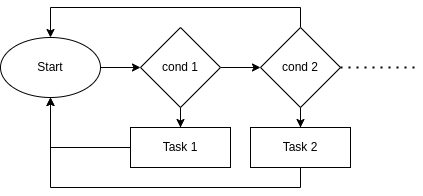
\includegraphics[width=0.5\textwidth]{images/chapter/implementation/Virtual timer.png}  % Adjust the width as necessary
    \caption{Virtual Timer Fluxogram}
    \label{fig:Virtual Timer Fluxogram}        
\end{figure}


The algorithm for this virtual timer goes for comparing the current elapsed time with the last value that the
"Task" was executed for each of them. Meaning, with an example, that if a task executes for each 500ms and other each 1000ms, both
can run without blocking the CPU.
